% Isolated author-review copy. The formal manuscript is not modified.
\documentclass[conference]{IEEEtran}

\usepackage{amsmath,amssymb}
\usepackage{booktabs}
\usepackage{graphicx}
\usepackage{tabularx}
\usepackage{stfloats}
\usepackage{capt-of}
\usepackage{url}
\usepackage{balance}
\setcounter{dbltopnumber}{2}
\renewcommand{\dbltopfraction}{0.95}
\renewcommand{\textfraction}{0.05}

\title{Measurement-Based Extraction and Statistical Modeling of GPS L1 C/A Multipath Components in Urban and Mountain/Valley Environments}

\author{\IEEEauthorblockN{Liang Feng}
\IEEEauthorblockA{Tongji University, Shanghai, China\\2432132@tongji.edu.cn}}

\begin{document}
\maketitle

\begin{abstract}
Multipath propagation in a time-varying satellite-to-ground channel produces delayed and Doppler-shifted replicas of the direct GPS signal. This paper presents a measurement-based method for extracting individual multipath components (MPCs) and establishing statistical models for Urban and Mountain/Valley environments. Navigation data are used to form coherent 40-ms observations for each tracked satellite. The space-alternating generalized expectation-maximization (SAGE) algorithm is applied to estimate the delay, Doppler, and complex gain of candidate MPCs. Based on temporal consistency across adjacent observations, stable estimates are selected for channel modeling. The analysis uses 518 persistent MPC observations from 236 satellite tracks. The excess-delay observations are right-skewed, relative power has two main modes, and signed relative Doppler is represented by a track-balanced empirical cumulative distribution. A shifted lognormal distribution is used for excess delay, and a two-component Gaussian mixture model is used for relative power. The decrease in relative power with excess delay is represented by two connected line segments with different slopes. Once an environment is specified, these models can generate random MPC parameter samples for simplified GNSS channel simulations and receiver evaluation.
\end{abstract}

\begin{IEEEkeywords}
GNSS multipath, GPS L1 C/A, SAGE, channel modeling, delay, Doppler.
\end{IEEEkeywords}

\section{Introduction}
Global Navigation Satellite Systems (GNSS) support vehicle navigation and intelligent transportation. A moving receiver observes a time-varying satellite-to-ground channel. Reflections from buildings, terrain, and vehicles produce signal replicas with different delays, Doppler shifts, and powers. These parameters vary as the receiver moves \cite{eissfeller1996gpsdynamic,mora1998multipath,beitler2015cmcd}.

Earlier GPS multipath studies have characterized receiver-level effects through carrier-to-noise-density ratio, pseudorange error, and carrier-phase error \cite{mora1998multipath,bilich2007snr,xie2011vehicular}. These quantities indicate changes caused by multipath, but they do not provide the delay, Doppler, and gain of individual MPCs. Path-level parameters are useful for statistical channel modeling and controlled receiver evaluation.

GNSS multipath models operate at different levels. Jost et al. modeled indoor pseudorange errors with a two-component Gaussian mixture, and Khider et al. applied this error model to multisensor positioning \cite{jost2010pseudorange,khider2013pseudorange}. These receiver-oriented models describe ranging error rather than individual propagation paths. Lehner and Steingass instead used measured reflection delay, power, duration, and Doppler to construct a time-varying land-mobile satellite channel \cite{lehner2005lms}. At the path-parameter level, SAGE estimates individual MPC parameters from complex baseband measurements by updating subsets of channel parameters in sequence \cite{fessler1994sage,fleury1999sage}. Gaussian mixtures provide a compact representation when a measured power distribution has more than one mode \cite{selim2016mog}.

This work combines per-satellite MPC extraction with environment-specific statistical modeling. First, navigation-data alignment forms coherent GPS L1 C/A observations for every tracked satellite. Second, the SAGE algorithm is applied to estimate MPC delay, Doppler, and complex gain, and temporal consistency is used to select persistent observations. Third, measurement-based descriptions are established for excess delay, signed relative Doppler, relative power, and the power--delay relation in Urban and Mountain/Valley environments. These descriptions provide MPC parameters for GNSS simulations. Section II describes the measurements and per-satellite processing, Section III presents MPC estimation and statistical modeling, and Section IV presents the resulting models.

\section{Measurements and Signal Processing}
\subsection{Measurement Setup}
The measurement system uses a TEST-TREE RF-Catcher V2 and a roof-mounted GNSS dome antenna. The antenna is right-hand circularly polarized and has a 40-dB active gain. The receiver records GPS L1 C/A at 1575.42 MHz \cite{gpsis200n2022}. The sampling rate is 10.23 MHz. Samples are stored as interleaved, little-endian, signed 16-bit I/Q values.

The measurements were collected while the vehicle traveled along two types of roads. Urban routes are surrounded by dense buildings, whereas Mountain/Valley routes pass through mountainous or valley terrain.

\subsection{Per-Satellite Multipath Processing}
Statistical modeling requires MPC observations from all available satellite-to-ground channels. GNSS-SDR first tracks each visible satellite and decodes its navigation data \cite{fernandez2011gnsssdr}. Because the satellites use different pseudorandom-noise codes, a separate signal stream is formed and processed for each satellite. Fig.~\ref{fig:workflow} summarizes this processing flow. Each GPS L1 C/A navigation bit lasts 20 ms, so a 40-ms observation can contain a bit transition that reverses the signal sign. The decoded bit signs are removed before coherent observations are formed. Correlation screening then identifies observations that may contain an additional signal component. For each selected observation, the SAGE algorithm is applied to estimate the parameters of the MPCs. Temporal consistency is evaluated afterward, and the resulting persistent MPC observations are combined across satellite tracks for statistical modeling.

\begin{figure*}[t]
\centering
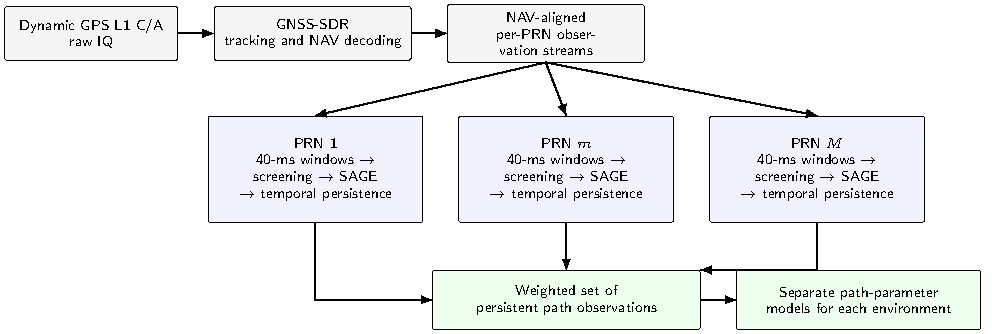
\includegraphics[width=0.96\textwidth]{figures/figure1_multisatellite.pdf}
\caption{Measurement and per-satellite MPC processing flow.}
\label{fig:workflow}
\end{figure*}

\section{Multipath Component Estimation and Statistical Modeling}
\subsection{SAGE-Based MPC Estimation}
Let $m$ denote one tracked satellite-to-receiver channel. Its complex baseband signal is
\begin{equation}
r_m(t)=\sum_{\ell=0}^{L_m-1}\alpha_{m,\ell}s_m(t-\tau_{m,\ell})
e^{j2\pi\nu_{m,\ell}t}+n_m(t),
\label{eq:signal}
\end{equation}
where $s_m(t)$ is the aligned C/A-code waveform and $n_m(t)$ is noise. MPC $\ell$ has complex gain $\alpha_{m,\ell}$, delay $\tau_{m,\ell}$, and Doppler frequency shift $\nu_{m,\ell}$. The earliest estimated component, indexed by $\ell=0$, is used as the reference component.

The SAGE algorithm updates one MPC at a time \cite{fessler1994sage,fleury1999sage}. For target MPC $\ell$, the E-step forms a conditional hidden-data estimate by subtracting the current contributions of the other MPCs from the received observation:
\begin{equation}
\mathbf r_{m,\ell}=\mathbf r_m-\sum_{k\ne\ell}\hat\alpha_{m,k}
\mathbf q_m(\hat\tau_{m,k},\hat\nu_{m,k}).
\label{eq:hidden}
\end{equation}
The M-step updates the delay and Doppler frequency shift of the target MPC by
\begin{equation}
(\hat\tau_{m,\ell},\hat\nu_{m,\ell})=
\operatorname*{arg\,max}_{\tau,\nu}
\frac{|\mathbf q_m(\tau,\nu)^H\mathbf r_{m,\ell}|^2}
{\mathbf q_m(\tau,\nu)^H\mathbf q_m(\tau,\nu)},
\label{eq:sage}
\end{equation}
where $\mathbf q_m(\tau,\nu)$ is a sampled code replica with fractional delay and Doppler. After all MPCs have been updated in one sweep, their complex gains are jointly estimated by least squares.

Equation~\eqref{eq:sage} selects the delay--Doppler pair with the highest normalized correlation to the conditional hidden-data estimate. A coarse correlation search provides the initial parameter values. The delay is then refined with fractional-sample code replicas spaced by 0.1 sample within a $\pm0.8$-sample neighborhood. The Doppler frequency shift is searched within $\pm30$ Hz of the tracking estimate in 5-Hz steps. The iterations terminate after 10 sweeps or when the relative change in the residual sum of squares (RSS) falls below $10^{-6}$.

For each 40-ms observation, SAGE is run with four possible path counts: one, two, three, and four MPCs. The path count is selected by comparing the Bayesian information criterion and residual error of the four results. This comparison balances signal representation against model complexity.

\subsection{Persistent MPC Observations}
MPC estimates from neighboring observations are compared after the local estimation. A match is declared only when the excess-delay, relative-Doppler, and relative-power differences are simultaneously no greater than 1.5 samples, 40 Hz, and 10 dB, respectively. An MPC is classified as persistent when matching estimates occur in at least three consecutive observations. A 40-ms observation is used for modeling only when every nonreference MPC satisfies this condition. The parameter values at the center time then form the persistent MPC observations.

For each persistent MPC observation, the three parameters are expressed relative to the reference component:
\begin{equation}
\Delta\tau=\tau_{\ell}-\tau_{0},\quad
\nu_{\rm rel}=\nu_{\ell}-\nu_{0},\quad
P_{\rm rel}=10\log_{10}\frac{|\alpha_{\ell}|^2}{|\alpha_{0}|^2}.
\label{eq:parameters}
\end{equation}
Here, $\Delta\tau$ is the delay relative to the reference component, $\nu_{\rm rel}$ is signed relative Doppler, and $P_{\rm rel}$ is the power relative to the reference component in decibels.

\subsection{Statistical Models for Each Environment}
The satellite tracks contain different numbers of retained observations. To prevent a long track from dominating the statistical analysis, every track is assigned the same total weight. If track $j$ contains $n_j$ observations, each observation in that track receives weight $w_i=1/n_j$.

Several parametric distributions were considered for excess delay and relative power in each environment. To compare them, one complete measurement scene was set aside. A model was estimated from all other scenes and evaluated on the set-aside scene. This process was repeated until every scene had been set aside once. Model selection used both the predictive likelihood and the maximum weighted CDF deviation,
\begin{equation}
D_w=\max_i\left|\widehat F_w(x_i)-F_\theta(x_i)\right|,
\label{eq:cdf-distance}
\end{equation}
where $\widehat F_w$ is the weighted empirical CDF and $F_\theta$ is the model CDF. A smaller $D_w$ indicates closer agreement between the measured and modeled cumulative distributions.

Signed relative Doppler is represented directly by its track-balanced empirical CDF. For environment $e$, the CDF and its weighted quantiles are defined as
\begin{equation}
\begin{aligned}
\widehat F_{\nu,e}(x)
&=\frac{\sum_{i\in e}w_i\mathbf{1}(\nu_i\le x)}
{\sum_{i\in e}w_i},\\
P_q(e)&=\inf\{x:\widehat F_{\nu,e}(x)\ge q\}.
\end{aligned}
\label{eq:doppler-ecdf}
\end{equation}
Here, $\nu_i$ is the signed relative Doppler of observation $i$. The empirical representation retains the measured Doppler values and is summarized by $P_{10}$, $P_{50}$, and $P_{90}$.

Because the excess-delay observations are positive and right-skewed, they are modeled by the lognormal form
\begin{equation}
\ln(\Delta\tau-\tau_s)\sim\mathcal N(\mu_\tau,\sigma_\tau^2),
\label{eq:lognormal}
\end{equation}
where $\tau_s$ is a shift, $\exp(\mu_\tau)$ is the scale, and $\sigma_\tau$ controls the spread in the logarithmic domain. The Urban model uses an estimated shift, while the Mountain/Valley model uses $\tau_s=0$.

The measured relative-power density contains two main modes. A two-component Gaussian mixture model (GMM) is therefore used for relative power:
\begin{equation}
p(x)=\pi\mathcal N(x;\mu_1,\sigma_1^2)
+(1-\pi)\mathcal N(x;\mu_2,\sigma_2^2).
\label{eq:gmm2}
\end{equation}
The mixing weight $\pi$ gives the relative contribution of the first Gaussian component. The two Gaussian terms represent the two modal regions in the relative-power measurements.

Relative power is also modeled as a function of excess delay. Two line segments with different slopes meet at a common breakpoint $\tau_b$:
\begin{equation}
P(\tau)=
\begin{cases}
P_b+b_1(\tau-\tau_b), & \tau<\tau_b,\\
P_b+b_2(\tau-\tau_b), & \tau\ge\tau_b.
\end{cases}
\label{eq:piecewise}
\end{equation}
This connected model allows the average rate of power decrease to change between low-delay and high-delay MPCs while preserving a continuous mean trend. After an environment is specified, excess delay and relative power can be sampled from their fitted distributions, while signed relative Doppler can be drawn from the corresponding weighted empirical CDF.

Receiver-level GPS multipath models describe quantities such as pseudorange error or carrier-to-noise-density ratio. Traditional land-mobile satellite channel models organize reflections in a time-varying channel impulse response or power-delay profile \cite{lehner2005lms}. The descriptions above provide extracted MPC delay, Doppler, and power together with their mean power--delay relation. They therefore provide measurement-based path parameters for simplified GNSS channel simulation and receiver evaluation.

The form of each model follows the main structure of the measured parameter. The lognormal density represents a positive delay with a long right tail. The two-component GMM represents the two modal regions in relative power. The empirical CDF retains the observed signed-Doppler values and their environment-specific concentration. The connected two-line model complements these marginal descriptions by describing how the mean relative power changes with delay. Using a common breakpoint keeps the power trend continuous while allowing different rates of change for shorter- and longer-delay MPCs.

\section{Statistical Modeling Results}
\begin{figure*}[!t]
\centering
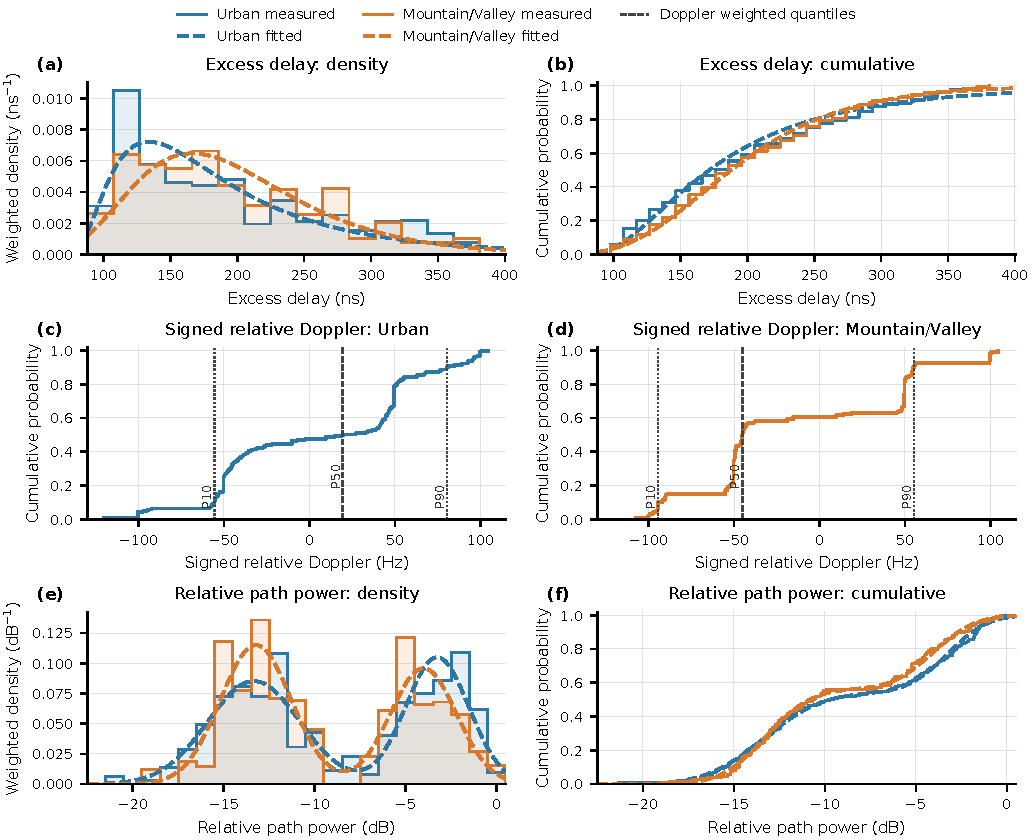
\includegraphics[width=0.98\textwidth]{../../figures/figure2_parameter_distributions.pdf}
\caption{Measured and modeled path-parameter distributions: (a)--(b) excess delay, (c)--(d) track-balanced empirical CDFs of signed relative Doppler for Urban and Mountain/Valley, respectively, and (e)--(f) relative path power. Fitted curves are shown for excess delay and relative power.}
\label{fig:path-distributions}
\end{figure*}

\subsection{Modeling Data and Excess Delay}
The analysis uses 518 persistent MPC observations from 236 satellite tracks, 36 recordings, and 9 measurement scenes. Of these observations, 346 are from Urban and 172 are from Mountain/Valley.

Fig.~\ref{fig:path-distributions}(a) and (b) show that both excess-delay distributions are right-skewed. The Urban fit has a shift of 68.7 ns, a scale of 102.8 ns, and a log-domain standard deviation of 0.675. The Mountain/Valley fit has a scale of 187.8 ns and a log-domain standard deviation of 0.348. The larger Urban spread represents its broader right tail. Table~\ref{tab:model-parameters} lists the model summaries and fit measures.

\subsection{Signed Relative Doppler}
Fig.~\ref{fig:path-distributions}(c) and (d) show the track-balanced empirical CDFs of signed relative Doppler. For Urban, the weighted $P_{10}$, $P_{50}$, and $P_{90}$ values are $-55.6$, $19.5$, and $80.6$ Hz, respectively. The corresponding values for Mountain/Valley are $-94.4$, $-45.1$, and $55.3$ Hz. The Mountain/Valley observations extend further toward negative Doppler, whereas the Urban observations are more evenly divided between negative and nonnegative values. The empirical CDF retains the measured concentration regions without introducing additional mixture components.

\subsection{Relative Power}
Fig.~\ref{fig:path-distributions}(e) and (f) show two relative-power modes in both environments. These values are relative to the earliest component and are not absolute received powers. The means are near $-13$ dB for the weaker mode and $-3$ to $-4$ dB for the stronger mode. The GMM reduces $D_w$ from 0.133 to 0.045 in Urban and from 0.137 to 0.037 in Mountain/Valley.

\subsubsection{Use in Channel Simulation}
The resulting descriptions provide statistical inputs for environment-specific Monte Carlo simulations. For a selected environment, the excess delay is drawn from its lognormal model, signed relative Doppler is drawn from the inverse of its weighted empirical CDF, and relative power is drawn from its two-component GMM. The power--delay model provides the corresponding mean power trend when delay dependence is required. The generated delay, Doppler, and relative power define the timing, frequency shift, and gain of an MPC in \eqref{eq:signal}. The same procedure can be repeated for each simulated satellite channel. Repeated draws produce random MPC combinations for evaluating GNSS signal processing and receiver algorithms.

\begin{table*}[!b]
\centering
\caption{Parameters of the models for each environment.}
\label{tab:model-parameters}
\scriptsize
\setlength{\tabcolsep}{3pt}
\begin{tabularx}{0.98\textwidth}{llXl}
\toprule
Quantity & Environment & Model summary & Fit measure\\
\midrule
Excess delay & Urban & Shifted lognormal: shift $68.7$ ns, scale $102.8$ ns, log-std. $0.675$ & $D_w=0.082$\\
& Mountain/Valley & Lognormal: scale $187.8$ ns, log-std. $0.348$ & $D_w=0.055$\\
Signed Doppler & Urban & Track-balanced empirical CDF: $P_{10}=-55.6$, $P_{50}=19.5$, $P_{90}=80.6$ Hz & ---\\
& Mountain/Valley & Track-balanced empirical CDF: $P_{10}=-94.4$, $P_{50}=-45.1$, $P_{90}=55.3$ Hz & ---\\
Relative power & Urban & GMM: $(-13.35,2.53,0.541)$ and $(-3.27,1.74,0.459)$ dB & $D_w=0.045$\\
& Mountain/Valley & GMM: $(-13.24,1.95,0.562)$ and $(-4.03,1.82,0.438)$ dB & $D_w=0.037$\\
Power--delay & Urban & Breakpoint $190.6$ ns; slopes $-3.53$ and $-5.57$ dB/100 ns & RMSE $4.01$ dB\\
& Mountain/Valley & Breakpoint $190.6$ ns; slopes $-6.31$ and $-4.46$ dB/100 ns & RMSE $3.44$ dB\\
\bottomrule
\end{tabularx}
\vspace{-1mm}
\parbox{0.98\textwidth}{\scriptsize For each GMM component, the three numbers are mean, standard deviation, and weight. $D_w$ is the maximum weighted CDF deviation defined in \eqref{eq:cdf-distance} and applies to the fitted delay and relative-power marginals. Signed Doppler is summarized by weighted empirical quantiles.}
\end{table*}

\twocolumn[{
\begin{minipage}{\textwidth}
\centering
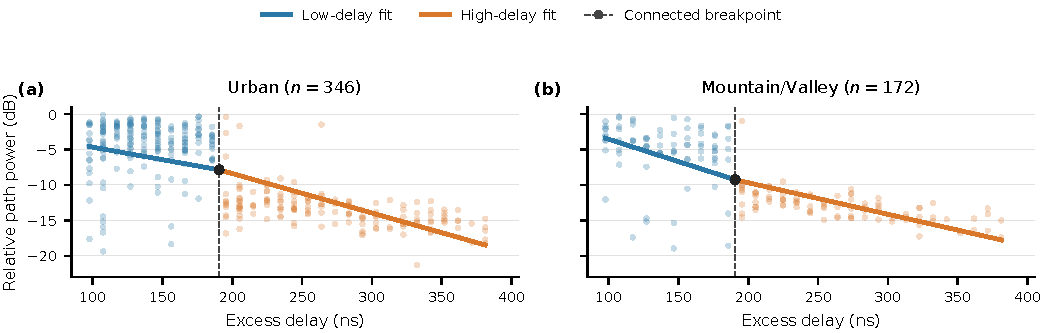
\includegraphics[width=0.94\textwidth]{../../figures/figure3_power_delay.pdf}
\captionof{figure}{Measured relative power and connected two-slope fits versus excess delay.}
\label{fig:power-delay}
\vspace{0.5em}
\end{minipage}
}]

\subsection{Power--Delay Relation}
Fig.~\ref{fig:power-delay} shows the decrease in relative power with increasing excess delay. The two fitted lines join at 190.6 ns. In Urban, the slopes are $-3.53$ and $-5.57$ dB per 100 ns before and after the breakpoint. In Mountain/Valley, they are $-6.31$ and $-4.46$ dB per 100 ns. Thus, the decrease becomes steeper after the breakpoint in Urban and less steep in Mountain/Valley. The root-mean-square errors are 4.01 and 3.44 dB, respectively.

\section{Conclusion}
This paper presents measurement-based extraction and statistical modeling of GPS L1 C/A MPCs from moving-vehicle measurements. Navigation-data alignment, per-satellite SAGE estimation, and temporal consistency provide persistent observations of excess delay, signed relative Doppler, and relative power. The resulting descriptions represent the right-skewed delay distribution, the observed signed-Doppler distributions, the two main modes of relative power, and the change in power-decay rate between low-delay and high-delay MPCs. Unlike receiver-level multipath indicators, these descriptions operate directly on individual MPC parameters. The fitted delay and power distributions can be sampled, and signed Doppler can be drawn from the corresponding empirical CDF, to generate environment-specific random MPC parameters for simplified GNSS channel simulations and receiver evaluation in Urban and Mountain/Valley propagation scenarios.

\balance
\bibliographystyle{IEEEtran}
\bibliography{references}

\end{document}
